\documentclass[12pt]{article}

\usepackage{graphicx}

\title{\bf{Paper reading for Voronoi Diagram in The Laguerre Geometry and its Applications}}
\date{}
\usepackage{CJK}
\begin{document}

\maketitle

\begin{CJK}{UTF8}{bkai}

\centerline{\bf 問題定義}

本問題想要在 {\it Laguerre geometry} 上求出 {\it Voronoi diagram}。\\

將一個三維空間的點~$(x,y,z)$~對應到歐氏平面上是一個半徑為~$|z|$~且圓心為~$(x,y)$~的圓,
而且此圓的旋轉方向是根據~$z$~的正負值,則稱為 {\it Laguerre geometry}。\\

在二維空間的一圓~$C_i=C_i(Q_i;r_i)$~,其中圓心為~$Q_i=(x_i,y_i)$~
,半徑為~$r_i$~。~$C_i$~和~$P=(x,y)$~之間的距離~$d_L(C_i,P)$~之定義如下:

\begin{equation}
d_L^2(C_i,P)=(x-x_i)^2+(y-y_i)^2-r_i^2
\end{equation}

因此,在 {\it Laguerre geometry} 上 $n$ 個圓 $C_i=C_i(Q_i;r_i)(Q_i=(x_i,y_i))$ 的 {\it Voronoi polygons} 的定義如下:

\begin{equation}
V(C_i)=\cap_i \{P \in R^2 | d_L^2(C_i,P) \leq d_L^2(C_j,P) \}
\end{equation}

求出所有的 {\it Voronoi polygons} ,就是我們要的 {\it Voronoi diagram}。\\


\centerline{\bf 方法說明}

%devide
假設一個 set $S=\{C_i(Q_i;r_i)|i=1,2,...,n\}$,我們要把 $S$ 分成兩個 subsets $L$ 和 $R$。也就是說,
根據所有 $Q_i$ 的 $x$ 座標大小找出中位數 $m$ ,再來分成兩個 subsets 如下式子:

\[
L=\{Q_i| x_i < m \},~R=\{Q_i| x_i \geq m \}
\]

分好之後,$L$ 和 $R$ 各自畫出它們的 {\it Voronoi diagram} ,再把兩個 {\it Voronoi diagram} 合併起來。\\

%merge

合併兩個 {\it Voronoi diagram} 之前,需要先找出兩者之間的 {\it dividing line}。 Dividing line
 是由兩個 {\it rays} 和多個 {\it line segments} 組成,所以第一個問題是要如何找出那兩個 rays。\\

%how to find the two rays ( see Lemma 7, or Lemma 5  )

一開始先建出 $L$ 和 $R$ 的 {\it convex hulls},它們的 convex hulls 分別是 CH($L$) 和 CH($R$),
然後再建出 $L \cup R$ 的 convex hulls CH($L \cup R$)。
把 CH($L \cup R$) 和另外兩個 convex hulls 做比較,就會發現有新的兩個 line segments 連接著
 CH($L$) 和 CH($R$)。
之後就從那兩個 line segments 求出兩個 rays。\\

從新生的 line segments 的特性觀察,發現有特性稱為 {\it degenerate}。所謂的 degenerate ,
是指新的 convex hull edges 與相鄰的舊的 convex hull edges 都在同一線上,如 Figure 1 所示:\\

%Fig. 5.(i)

\begin{figure}[h]
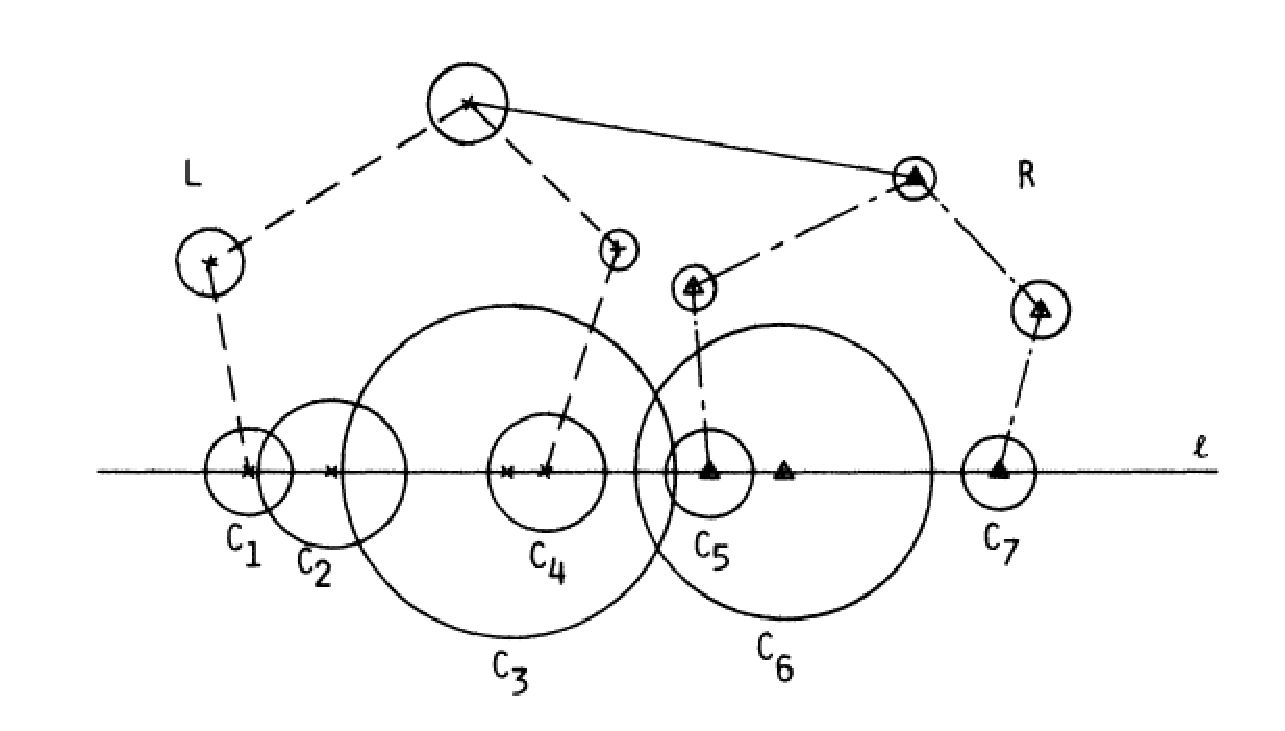
\includegraphics[scale=0.5]{figure5(i).eps}
\caption{}
\label{}
\end{figure}

明顯地, Figure 1 上某些新舊 convex hull edges 都在 $l$ 線上。在 Figure 1 中上面實線部份(非 $l$ 線段),就是沒有 degenerate
 特性的例子。如果是沒有 degenerate 的特性,只要在 $l$ 上 $L$ 與 $R$ 中最接近的兩點取 {\it radical axis}
 即可;degenerate 的例子,則需要把 $l$ 分成 $L_l \subseteq L$ 和 $R_l \subseteq R$兩個集合。將兩個 Voronoi
 diagram $V(L_l)$ 和 $V(R_l)$ 合併,方法就類似兩個排序好的 list 合併成一個排序好的 list 。也就是說,將 $V(L_l)$
 和 $V(R_l)$ 中的 Voronoi edges 依照由左到右排序好,並且合併起來,如圖 Figure 2:

%insert the picture Fig. 5(iv)

\begin{figure}[h]
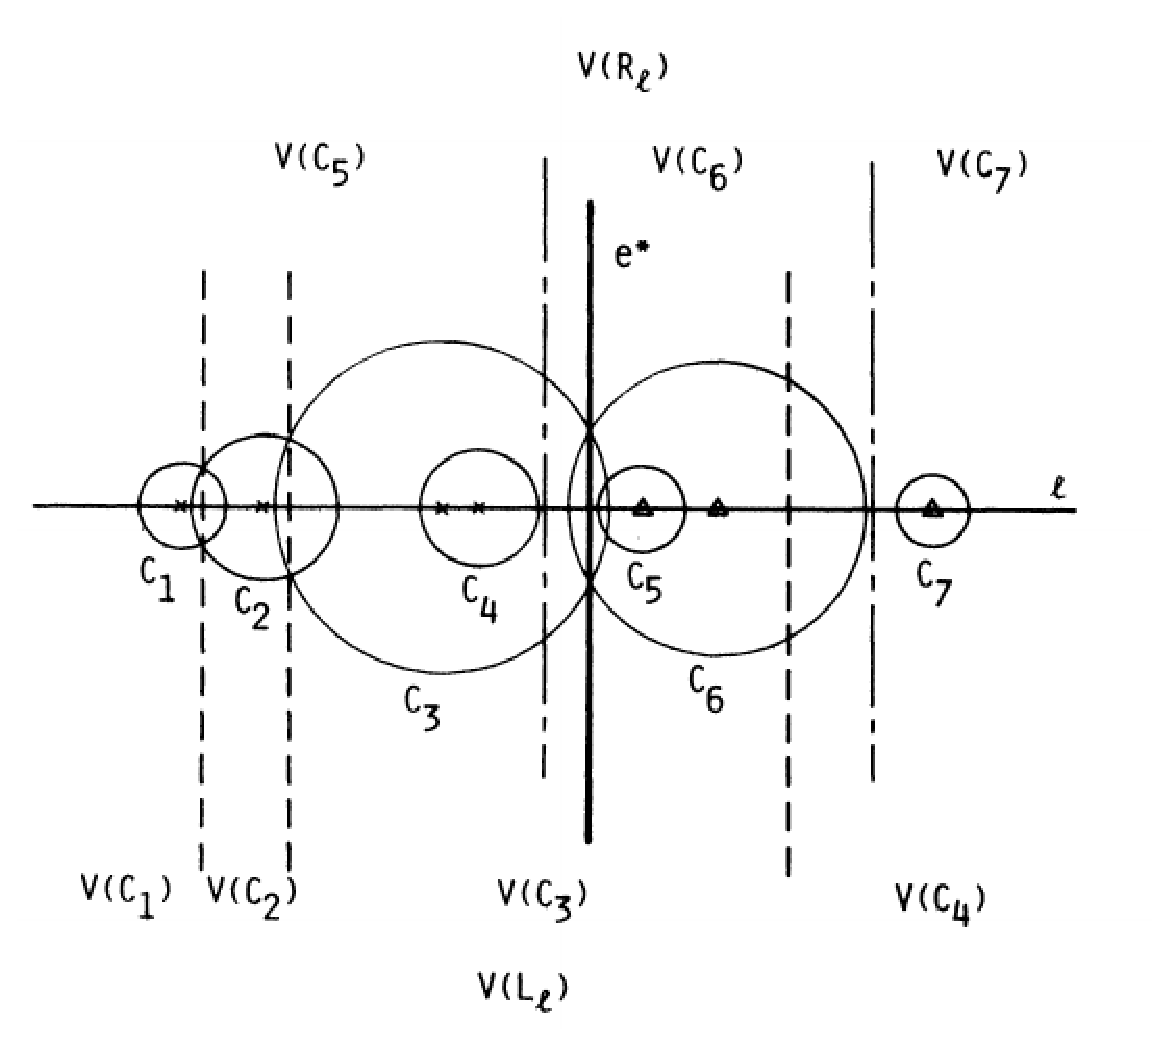
\includegraphics[scale=0.5]{figure5(iv).eps}
\caption{}
\label{}
\end{figure}

在 Figure 2 中,每相鄰兩個 Voronoi edges 夾出的區域為 $V(L_l)$ 中某個 Voronoi polygon $V(C_i)$ 和 $V(R_l)$ 中某個 Voronoi polygon
 $V(C_j)$ 的交集。因此,我們只需要求每個 $C_i$ 與 $C_j$ 的 radical axis,是否落在它們交集的區域內;若符合上述條件,則
那個 radical axis 是我們要的 ray。

%how to trace the several line segments ( see Lemma 4, and refer.[9]  )

從這兩條 rays 往圖形內部延伸,並且不斷地去做順時鐘方向和逆時鐘方向去調整,方法與歐式平面上的演算法相同。
當兩個 rays 連在一起,就形成我們要的 dividing line 。\\



\centerline{\bf 例子}

Figure 3 上的 13 個圓為初始輸入,演算法步驟如下:

\begin{enumerate}

\item 找出 13 個圓心在 x 軸上的中位數,並且分開來,如 Figure 4 。
\item 左右兩邊繼續切割,直到剩下一個或兩個點就停止切割,如 Figure 5 。
\item 兩邊分別畫出各自的 Voronoi diagram 之後,就開始合併兩邊的 diagram
最後如 Figure 6 。
\item 左右兩邊畫出各自的 convex hull ,再將兩邊的 convex hull 合併,如 Figure 7 。
\item Figure 7 中 $l_1$ 不為 degenerate case ,所以直接求 radical axis 即可,如
 Figure 8 。
\item $l_2$ 為 degenerate case ,所以將與 $l_2$ 共線的一起討論,如 Figure 9 。
\item 將與 $l_2$ 垂直的所有 Voronoi edges 合併並有左到右排序好,如 Figure 10 。
\item 在 Figure 10 中兩兩相鄰的 Voronoi edges 的區域由左到右分別是 $V(C_1)$ 和 $V(C_5)$ 的交集、
 $V(C_2)$ 和 $V(C_5)$ 的交集、$V(C_3)$ 和 $V(C_5)$ 的交集、 $V(C_3)$ 和 $V(C_6)$ 的交集
、$V(C_4)$ 和 $V(C_6)$、$V(C_4)$ 和 $V(C_7)$ 的交集。
\item 對每一個區域所對應的兩個圓求出 radical axis ,看是否落在對應的區域內。做完發現
 $V(C_3)$ 和 $V(C_6)$ 的 radical axis 有落在區間內,所以 ray 就求出來了,如 Figure 11 。
\item 兩個 rays 求完好後,就接著求出 dividing line 中間的 line segments 。方法就是先將某一條
 ray 往內延伸,每延伸到要超出某個 Voronoi polygon 時,就讓 ray 轉向,直到與另一的 ray 接在一起,如 Figure 12 。
\item 最後結果如 Figure 13 。

\end{enumerate}

\centerline{\bf 時間複雜度分析}

此演算法有三大部份:{\it divide} 、 {\it conquer} 、和 {\it merge} 。假設時間複雜度為 $T(n)$,
那三大部份的時間複雜度分析如下:\\

\begin{enumerate}
\item {\it divide} :$O(n)$\\
\item {\it conquer} : $2T(n/2)$\\
\item {\it merge} : $O(n)$\\
\end{enumerate}

所以總時間複雜度 $T(n)=2T(n/2)+2O(n)=O(n\log n)$ 。


%Fig 3
\begin{figure}[h]
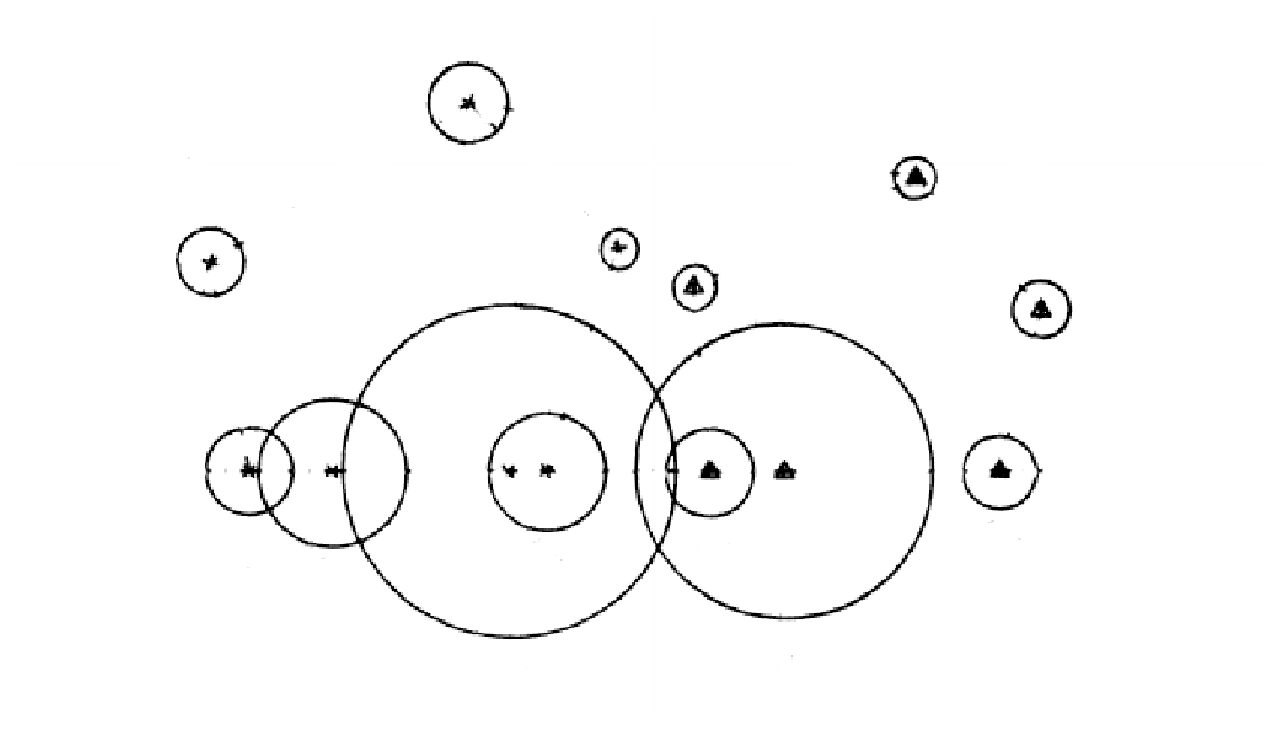
\includegraphics[scale=0.4]{figure3.eps}
\caption{}
\end{figure}

%Fig 4
\begin{figure}[h]
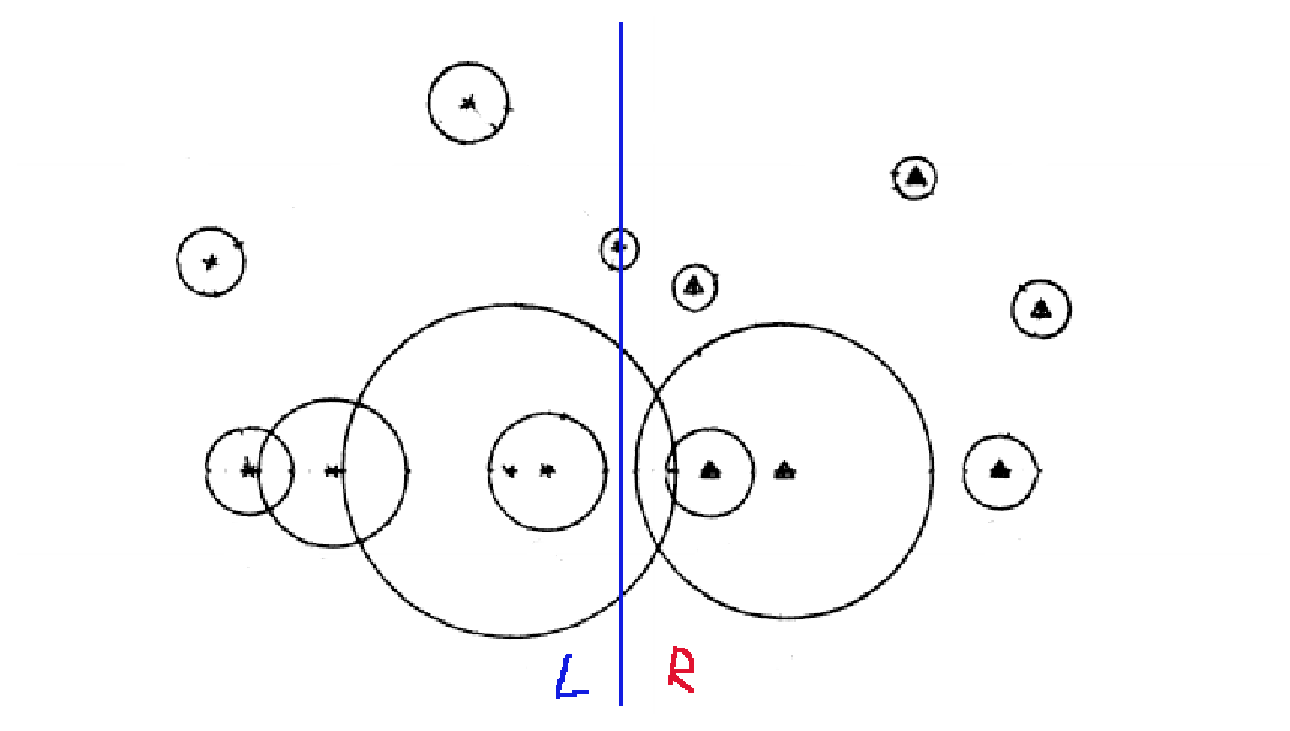
\includegraphics[scale=0.4]{figure4.eps}
\caption{}
\end{figure}

%Fig 5
\begin{figure}[h]
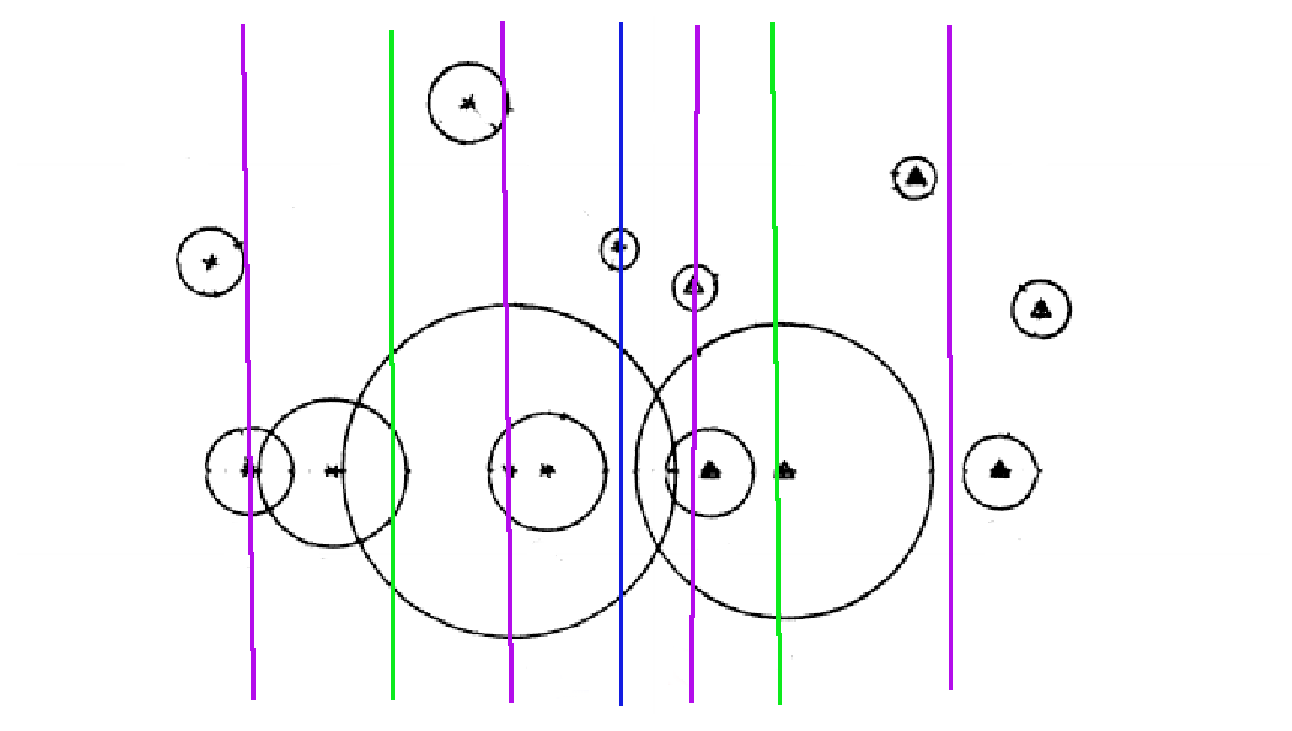
\includegraphics[scale=0.4]{figure5.eps}
\caption{}
\end{figure}

\end{CJK}

\end{document}
